%%%%%%%%%%%%%%%%%%%%%%%%%%%%%%%%%%%%%%%%%%%%%%%%%%
%%%%%%%%%%

% Figures

\begin{figure}[t]
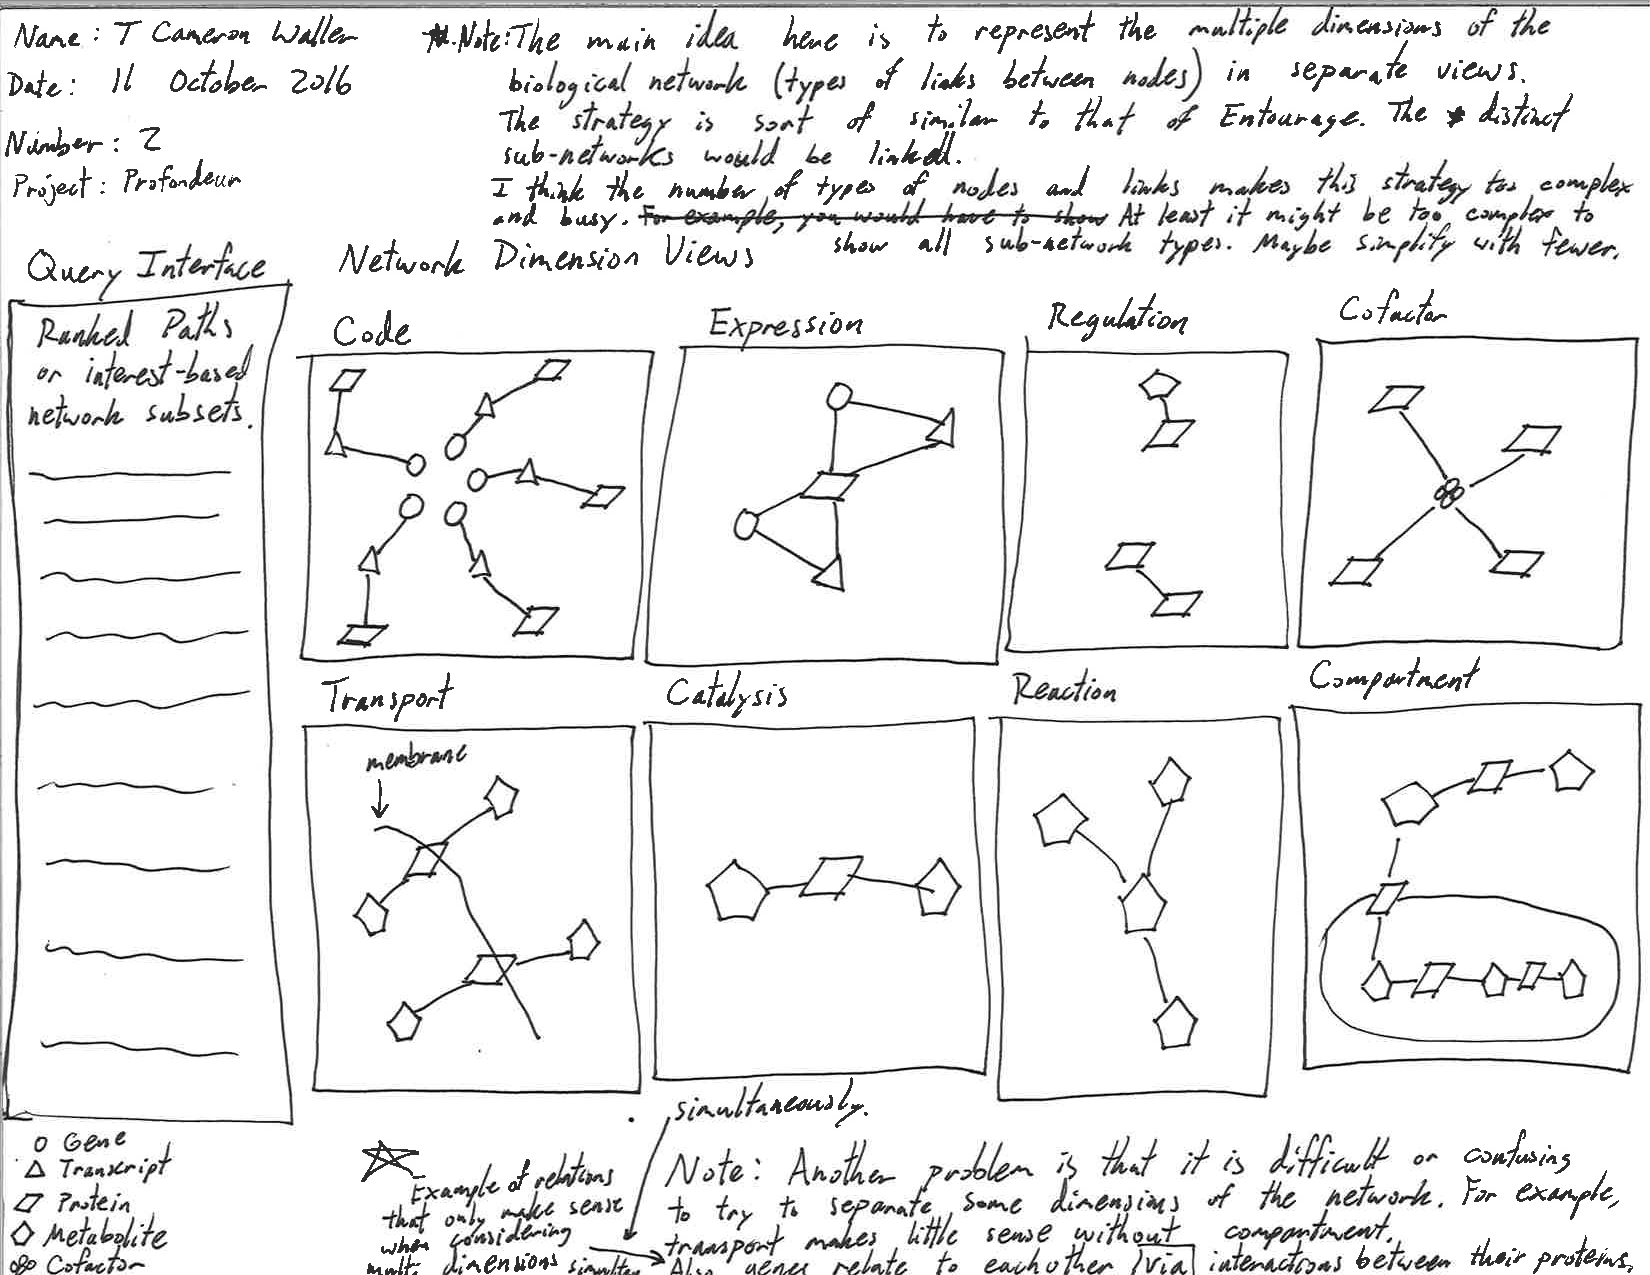
\includegraphics[scale=0.5]{sketch_2016-10-11_2}
\centering
\caption{Representations for multiple types of relations between multiple types of entities}
\label{fig:2016-10-11_2}
\end{figure}

\begin{figure}[t]
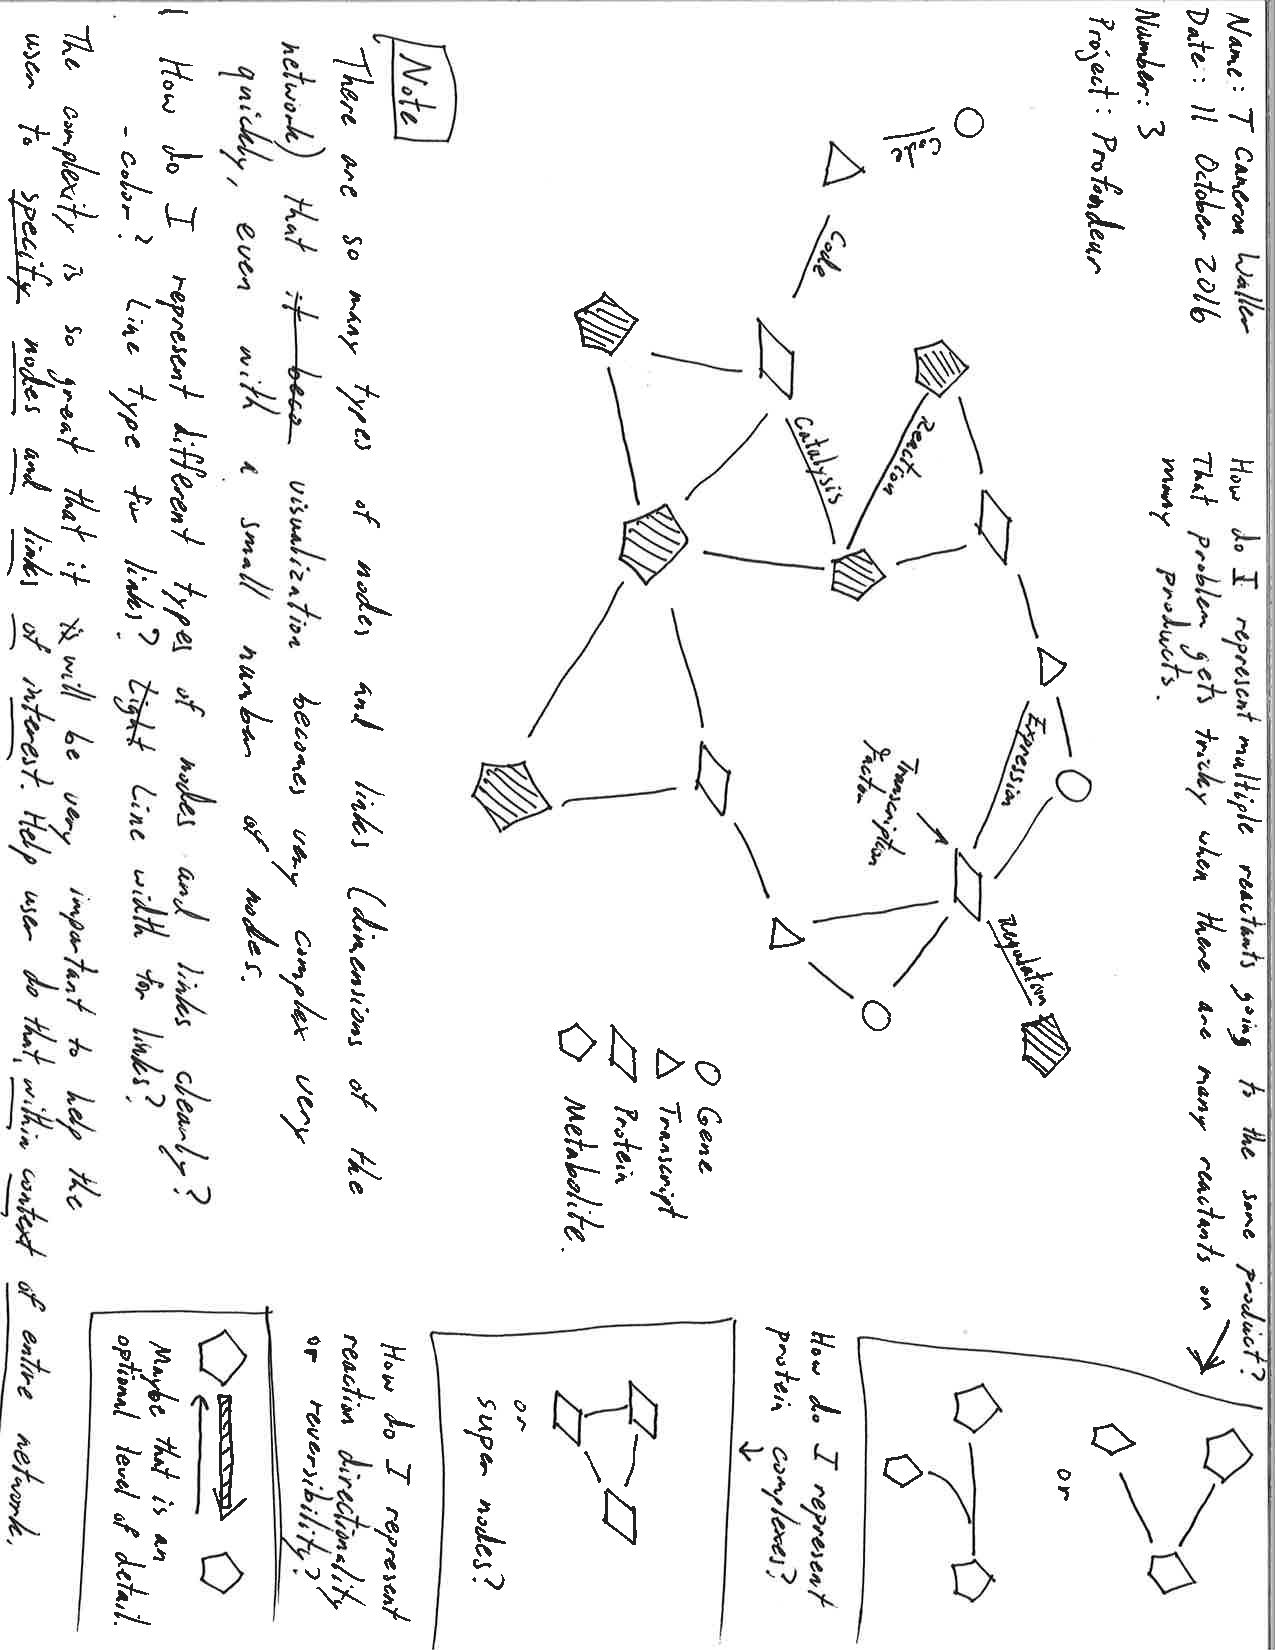
\includegraphics[scale=0.5]{sketch_2016-10-11_3}
\centering
\caption{Representations for multiple types of relations between multiple types of entities}
\label{fig:2016-10-11_3}
\end{figure}

\begin{figure}[t]
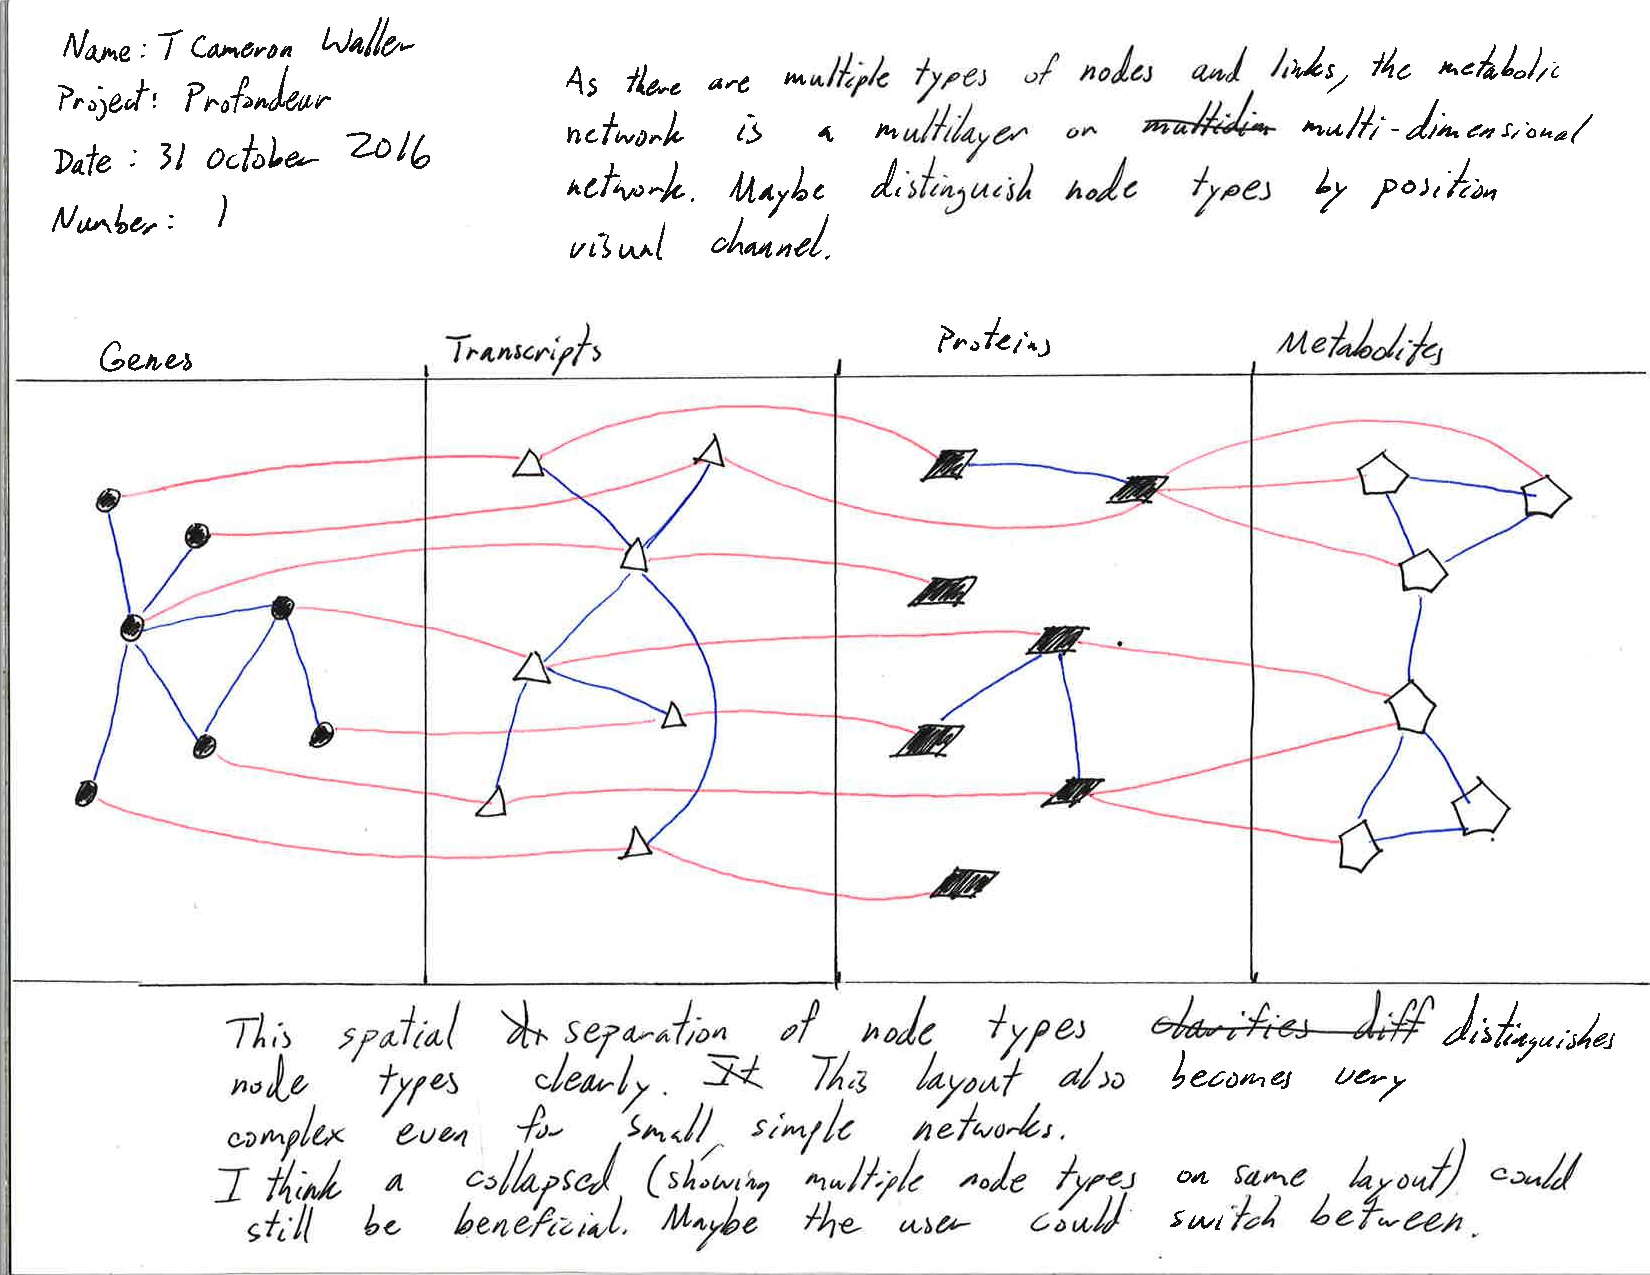
\includegraphics[scale=0.5]{sketch_2016-10-31_1}
\centering
\caption{Representations for multiple types of relations between multiple types of entities}
\label{fig:2016-10-31_1}
\end{figure}

\begin{figure}[t]
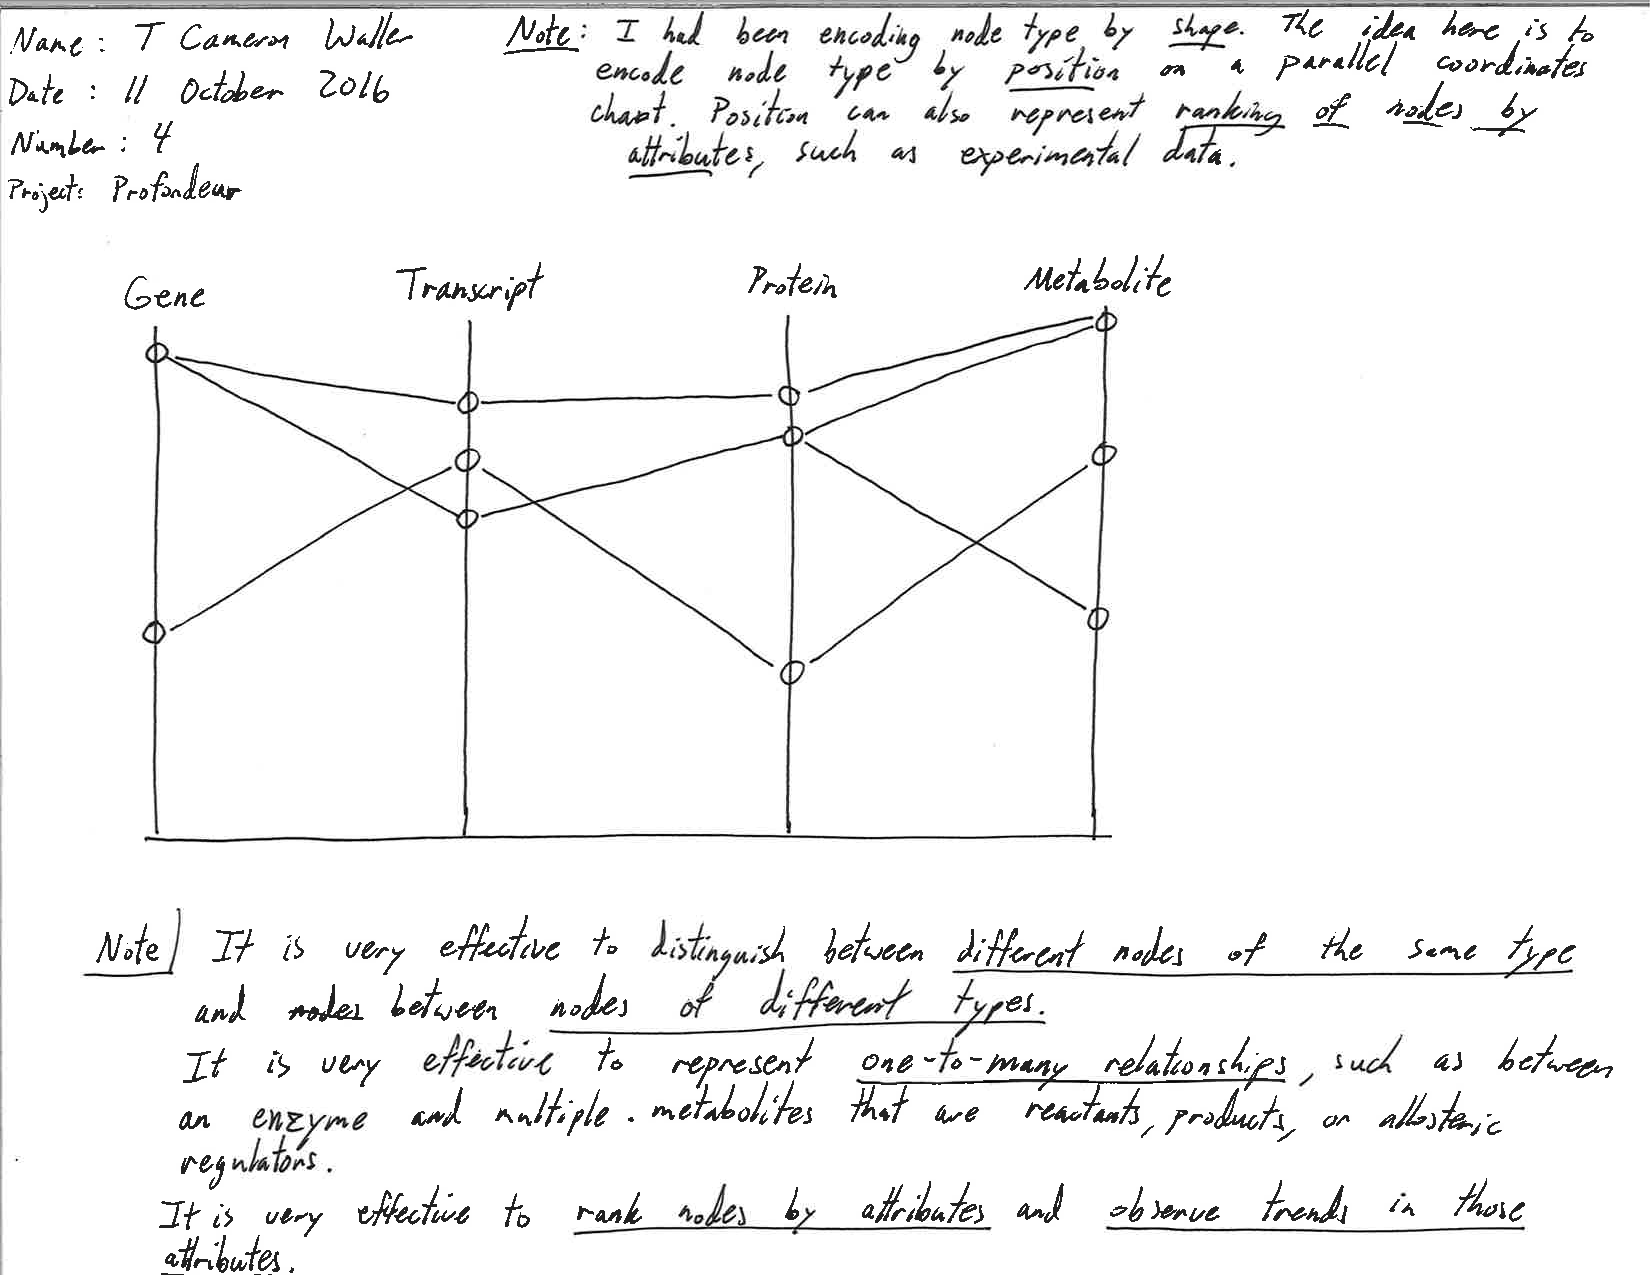
\includegraphics[scale=0.5]{sketch_2016-10-11_4}
\centering
\caption{Alternative representation with parallel coordinates chart}
\label{fig:2016-10-11_4}
\end{figure}

\begin{figure}[t]
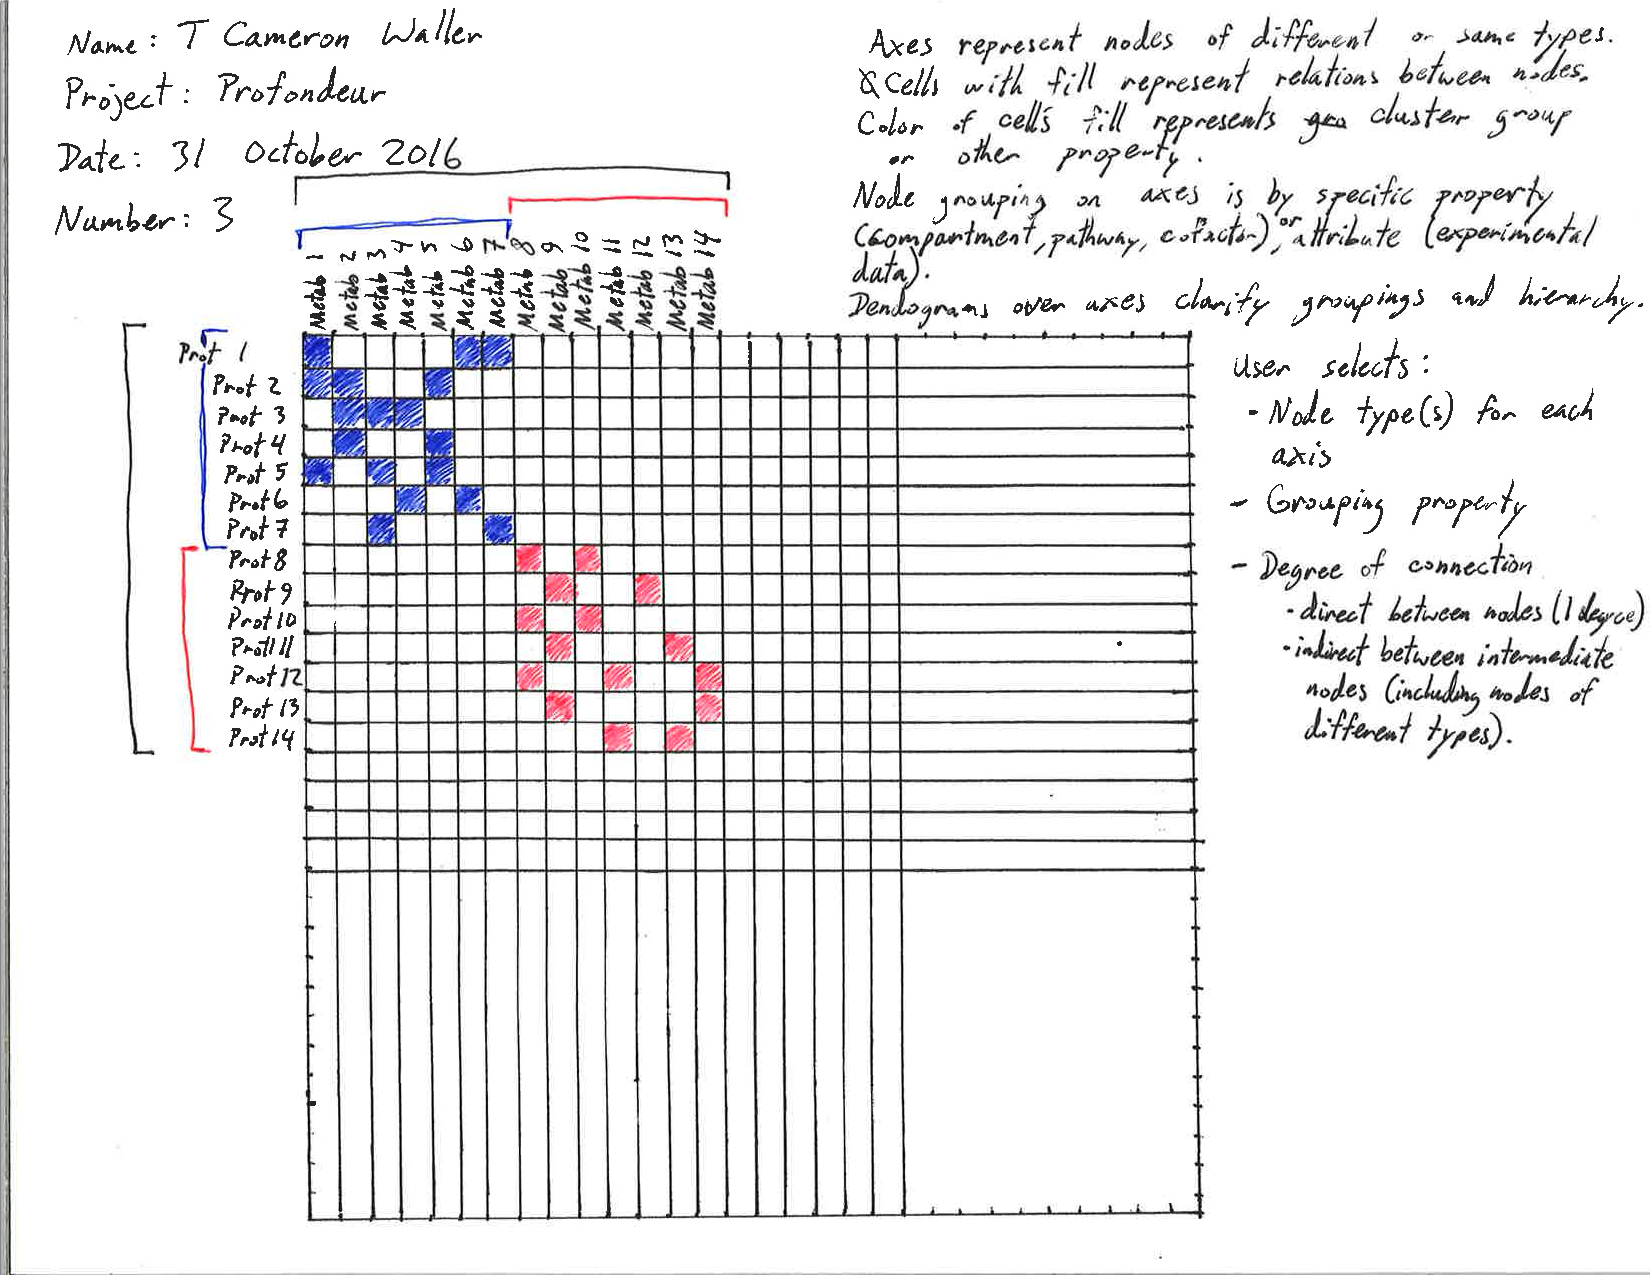
\includegraphics[scale=0.5]{sketch_2016-10-31_3}
\centering
\caption{Alternative representation with matrix or grid chart}
\label{fig:2016-10-31_3}
\end{figure}

\begin{figure}[t]
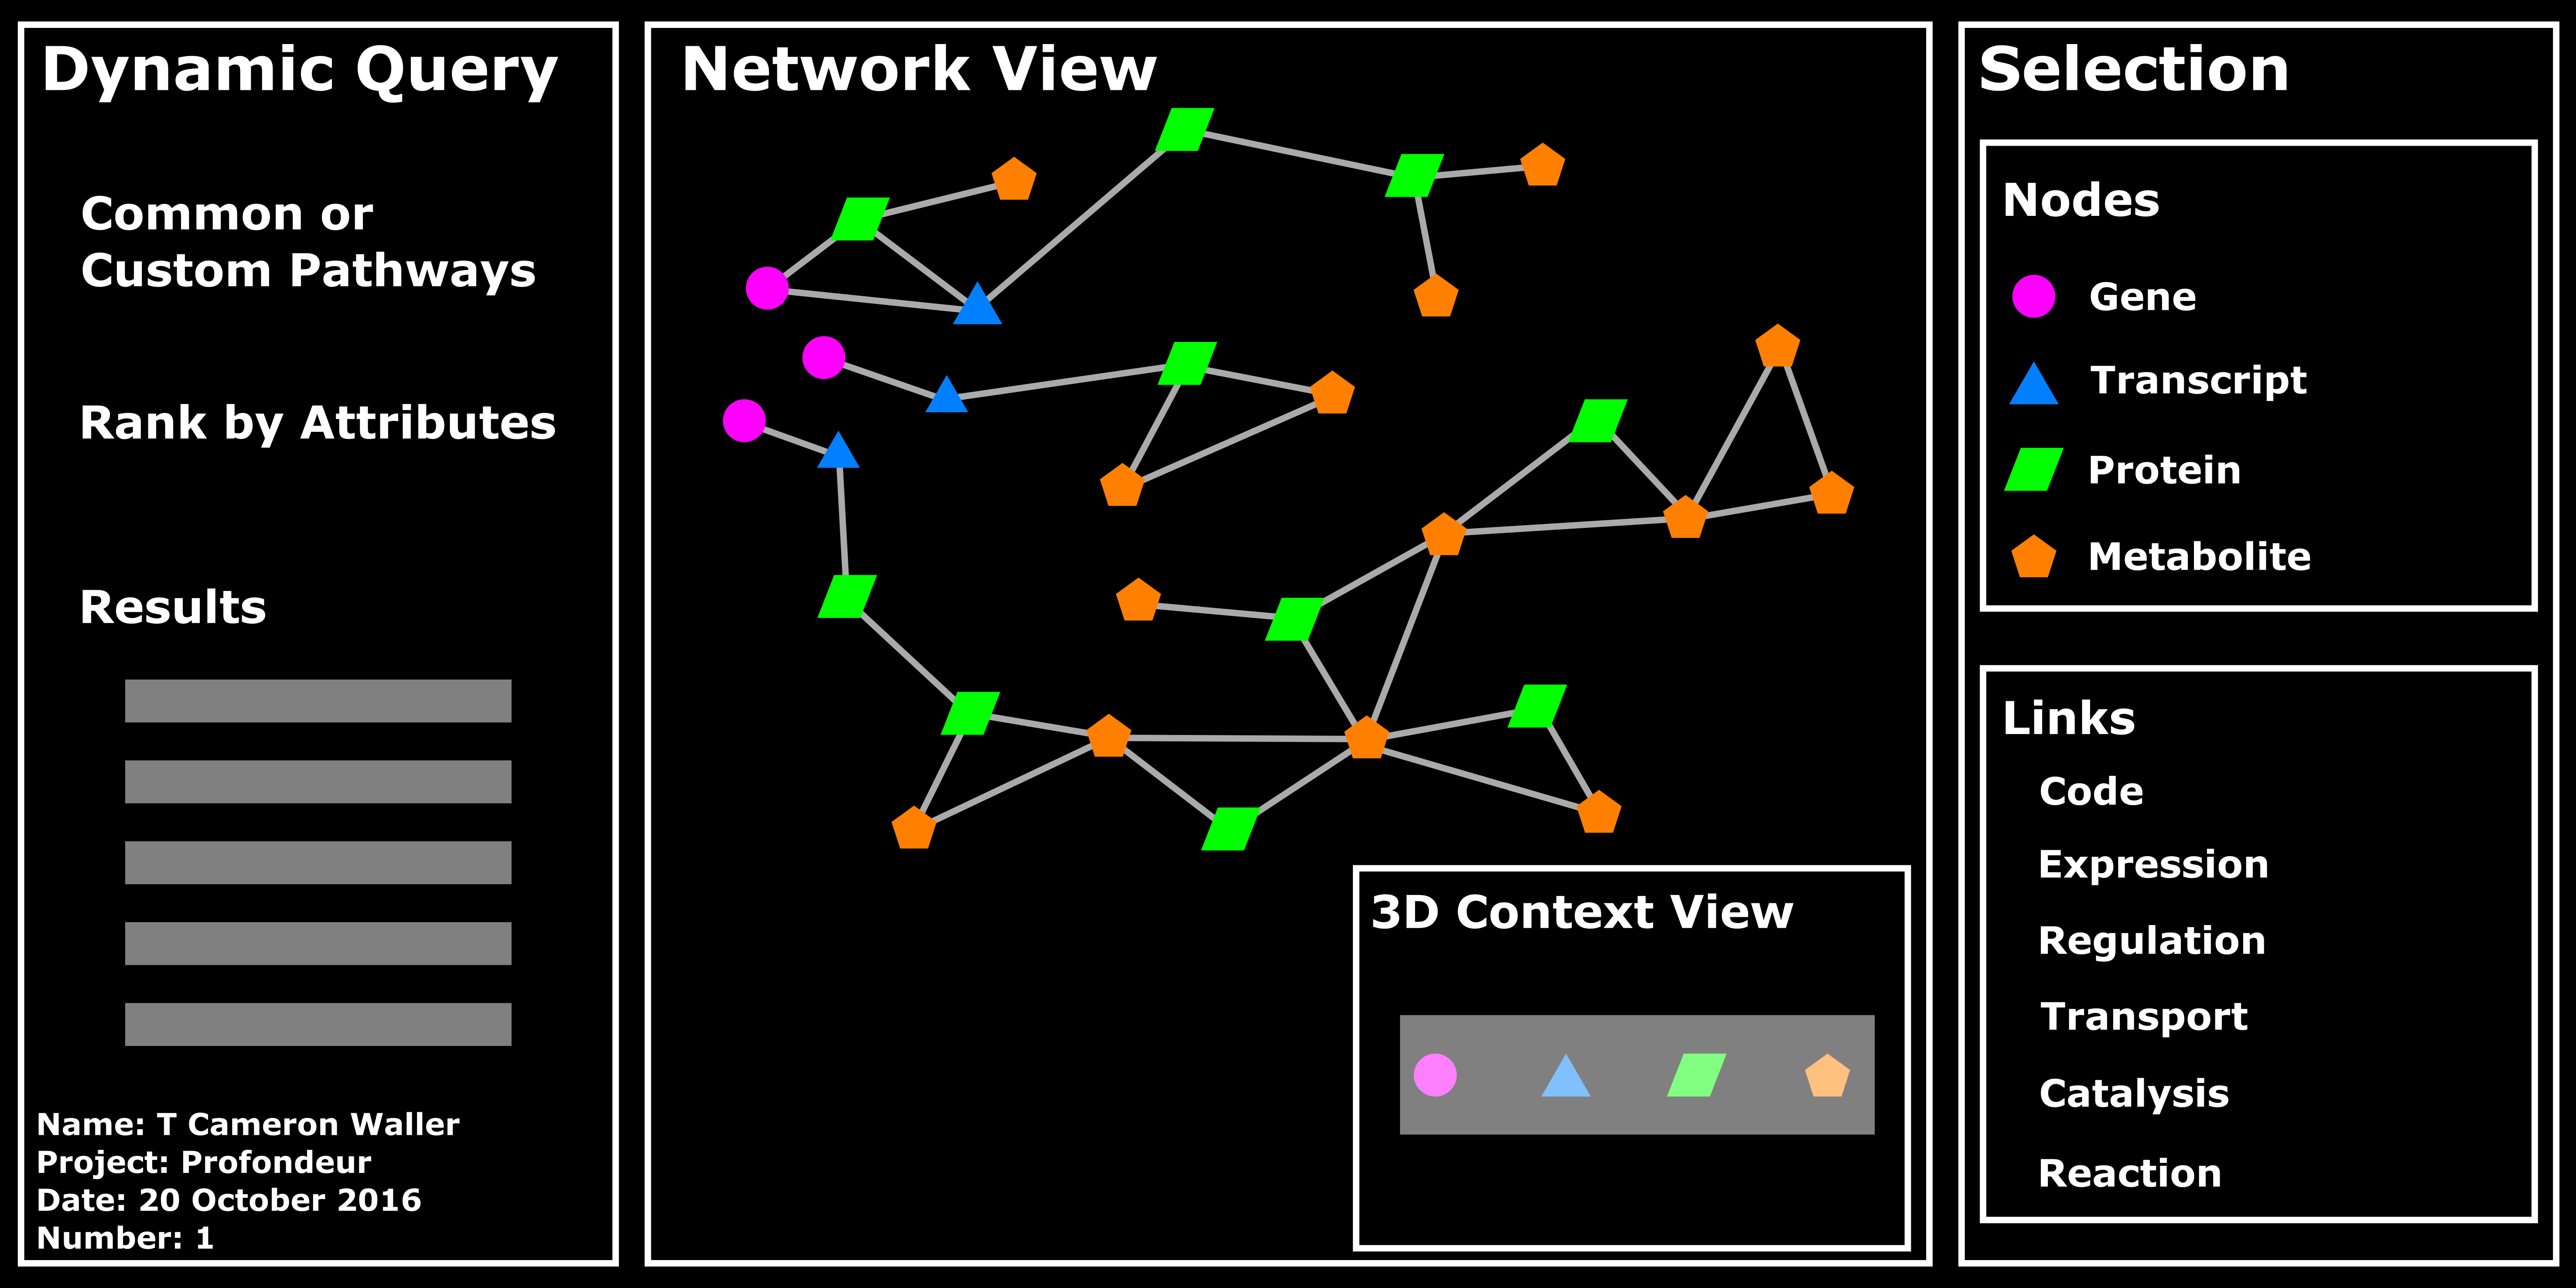
\includegraphics[scale=0.4]{sketch_2016-10-20_1}
\centering
\caption{Early idea for interface design}
\label{fig:2016-10-20_1}
\end{figure}

\begin{figure}[t]
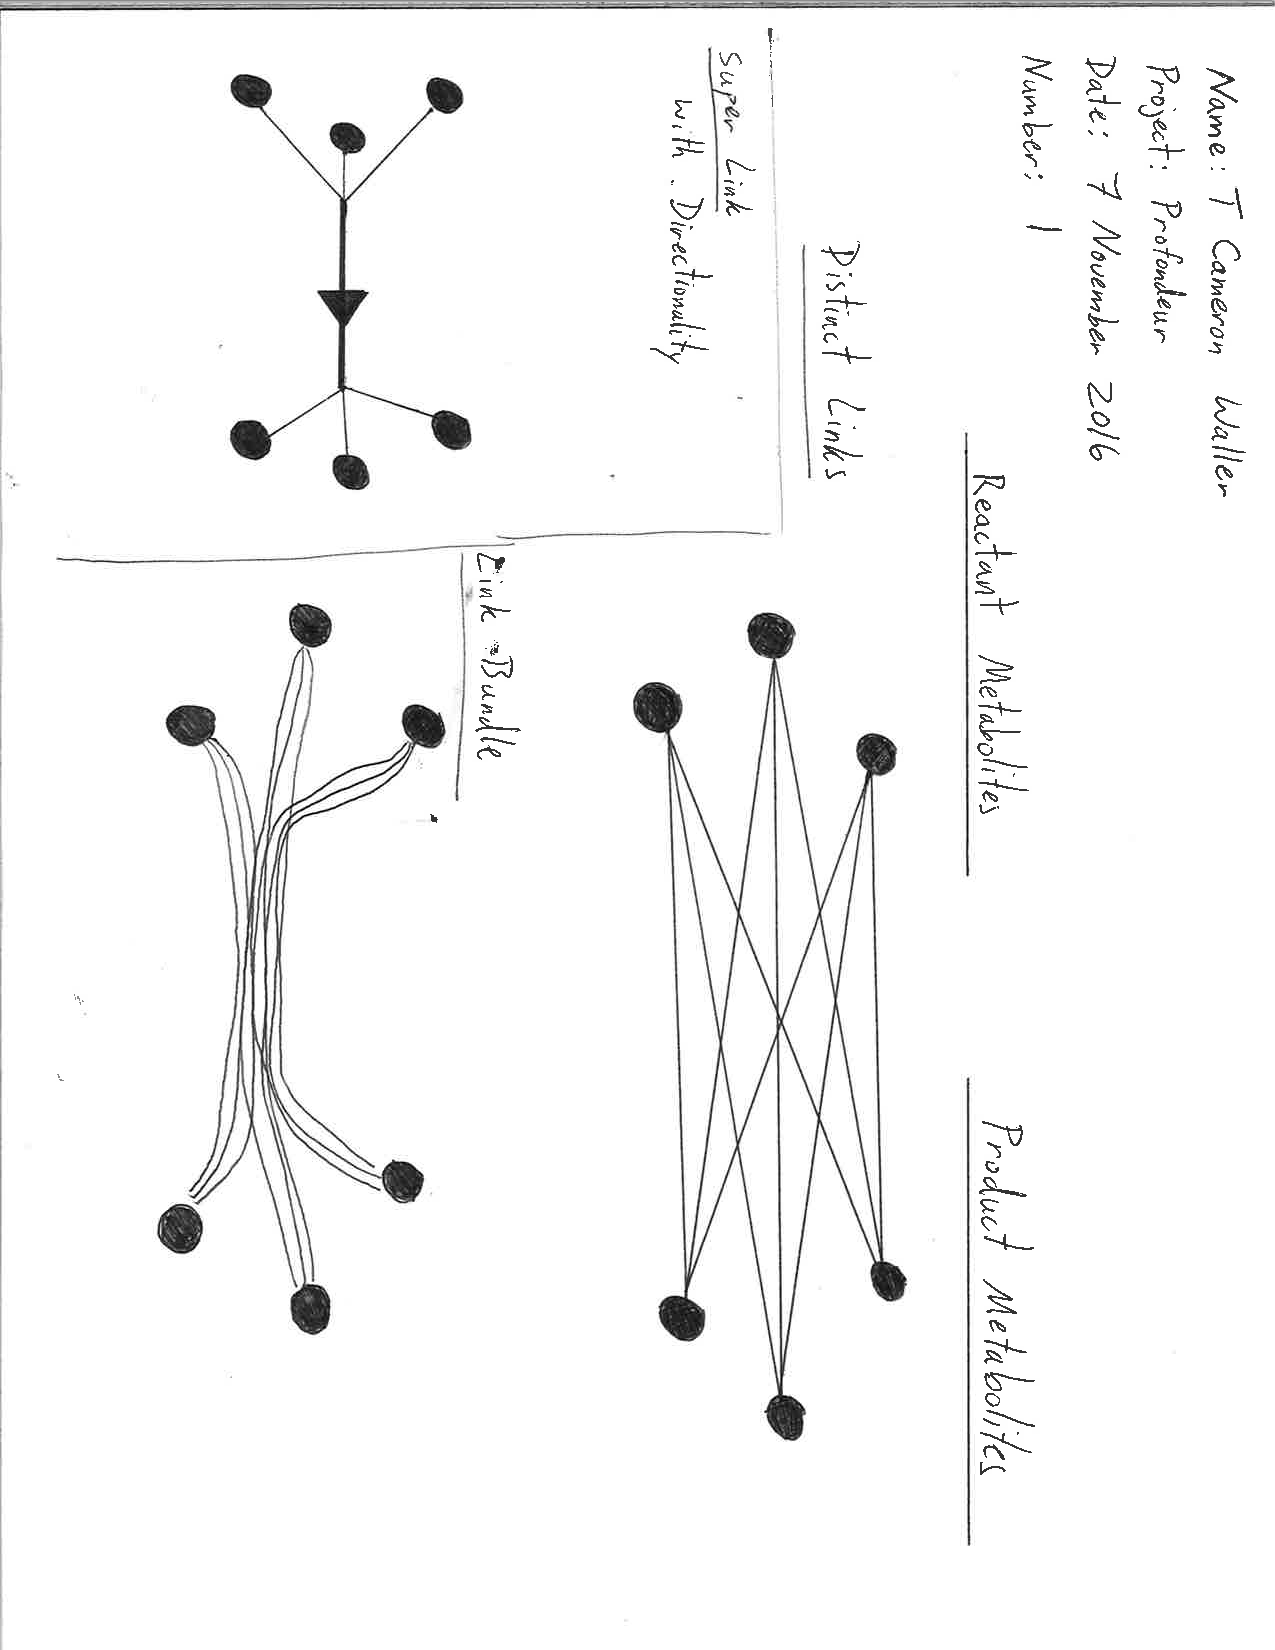
\includegraphics[scale=0.5]{sketch_2016-11-07_1}
\centering
\caption{Link bundles and super links for reactions between metabolite nodes}
\label{fig:2016-11-07_1}
\end{figure}

\begin{figure}[t]
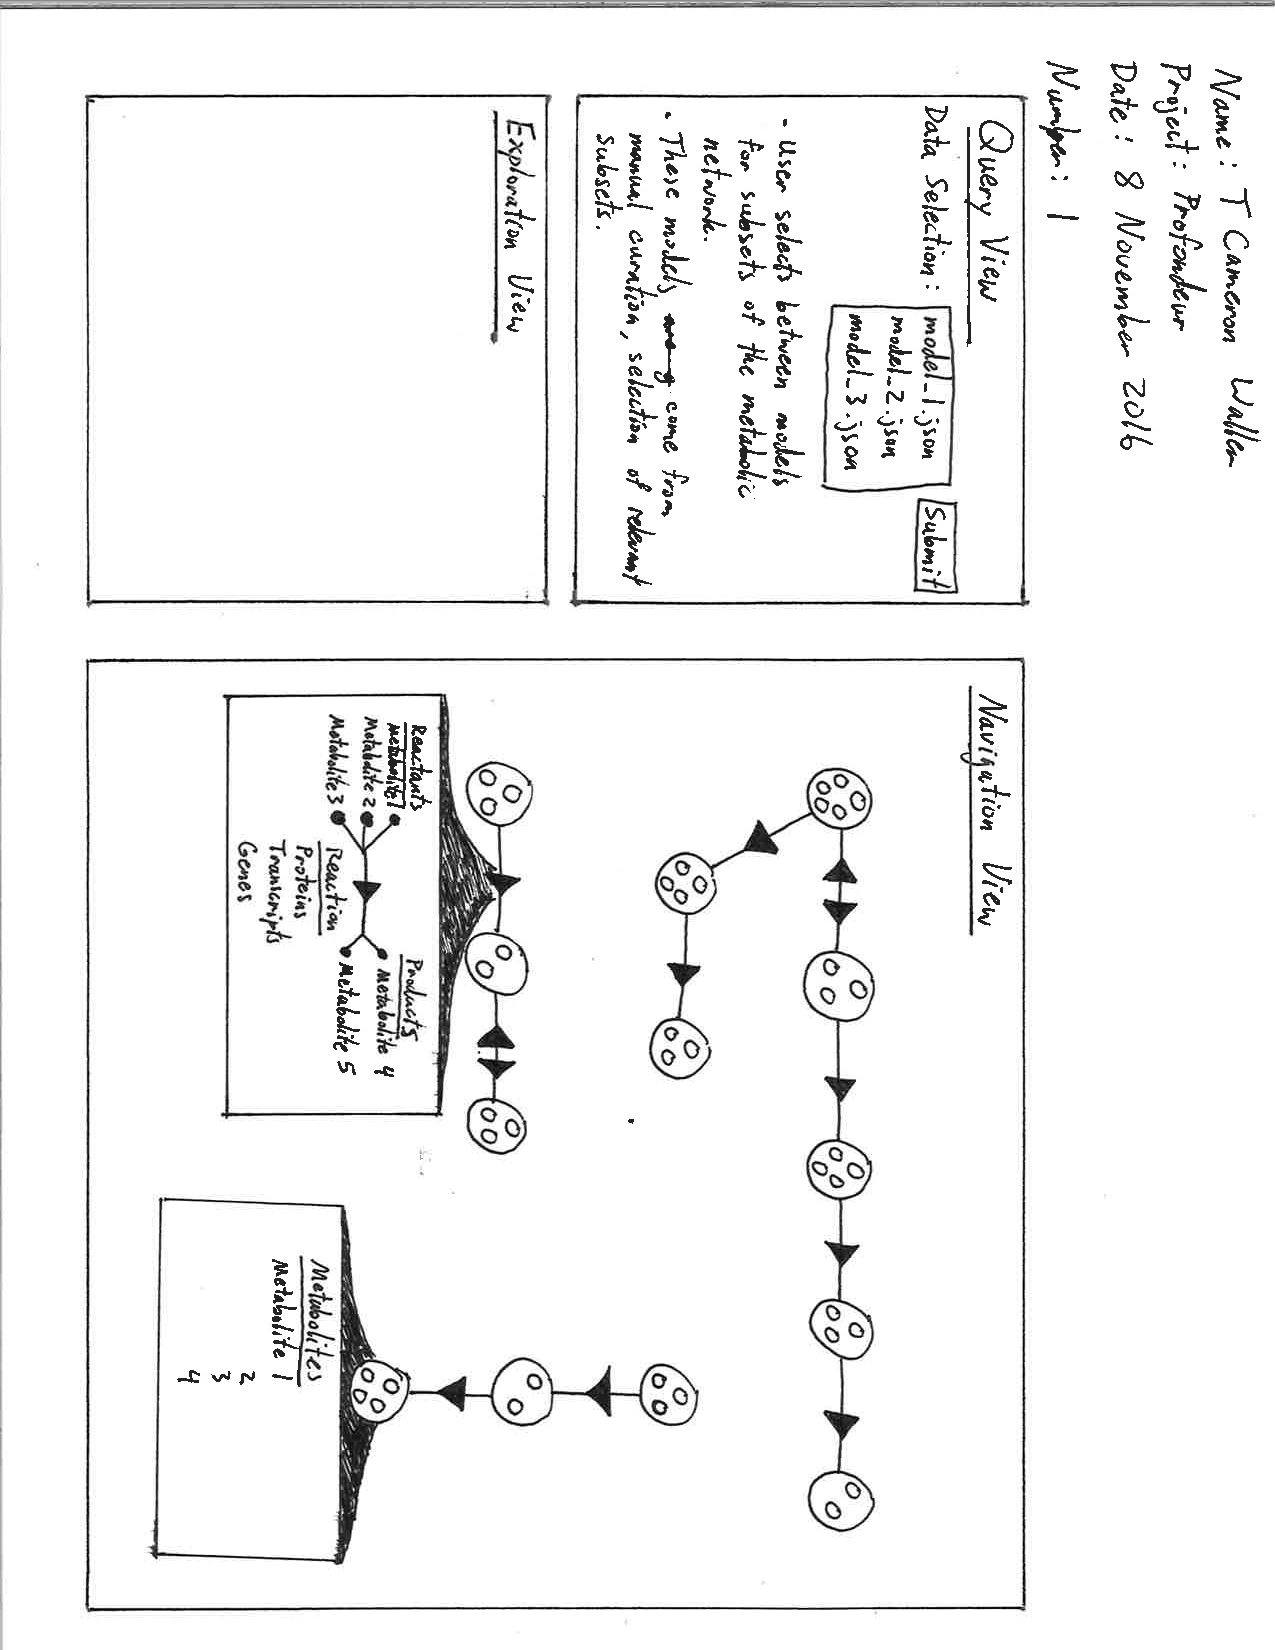
\includegraphics[scale=0.5]{sketch_2016-11-08_1}
\centering
\caption{Super nodes for reactant and product metabolites}
\label{fig:2016-11-08_1}
\end{figure}

\begin{figure}[t]
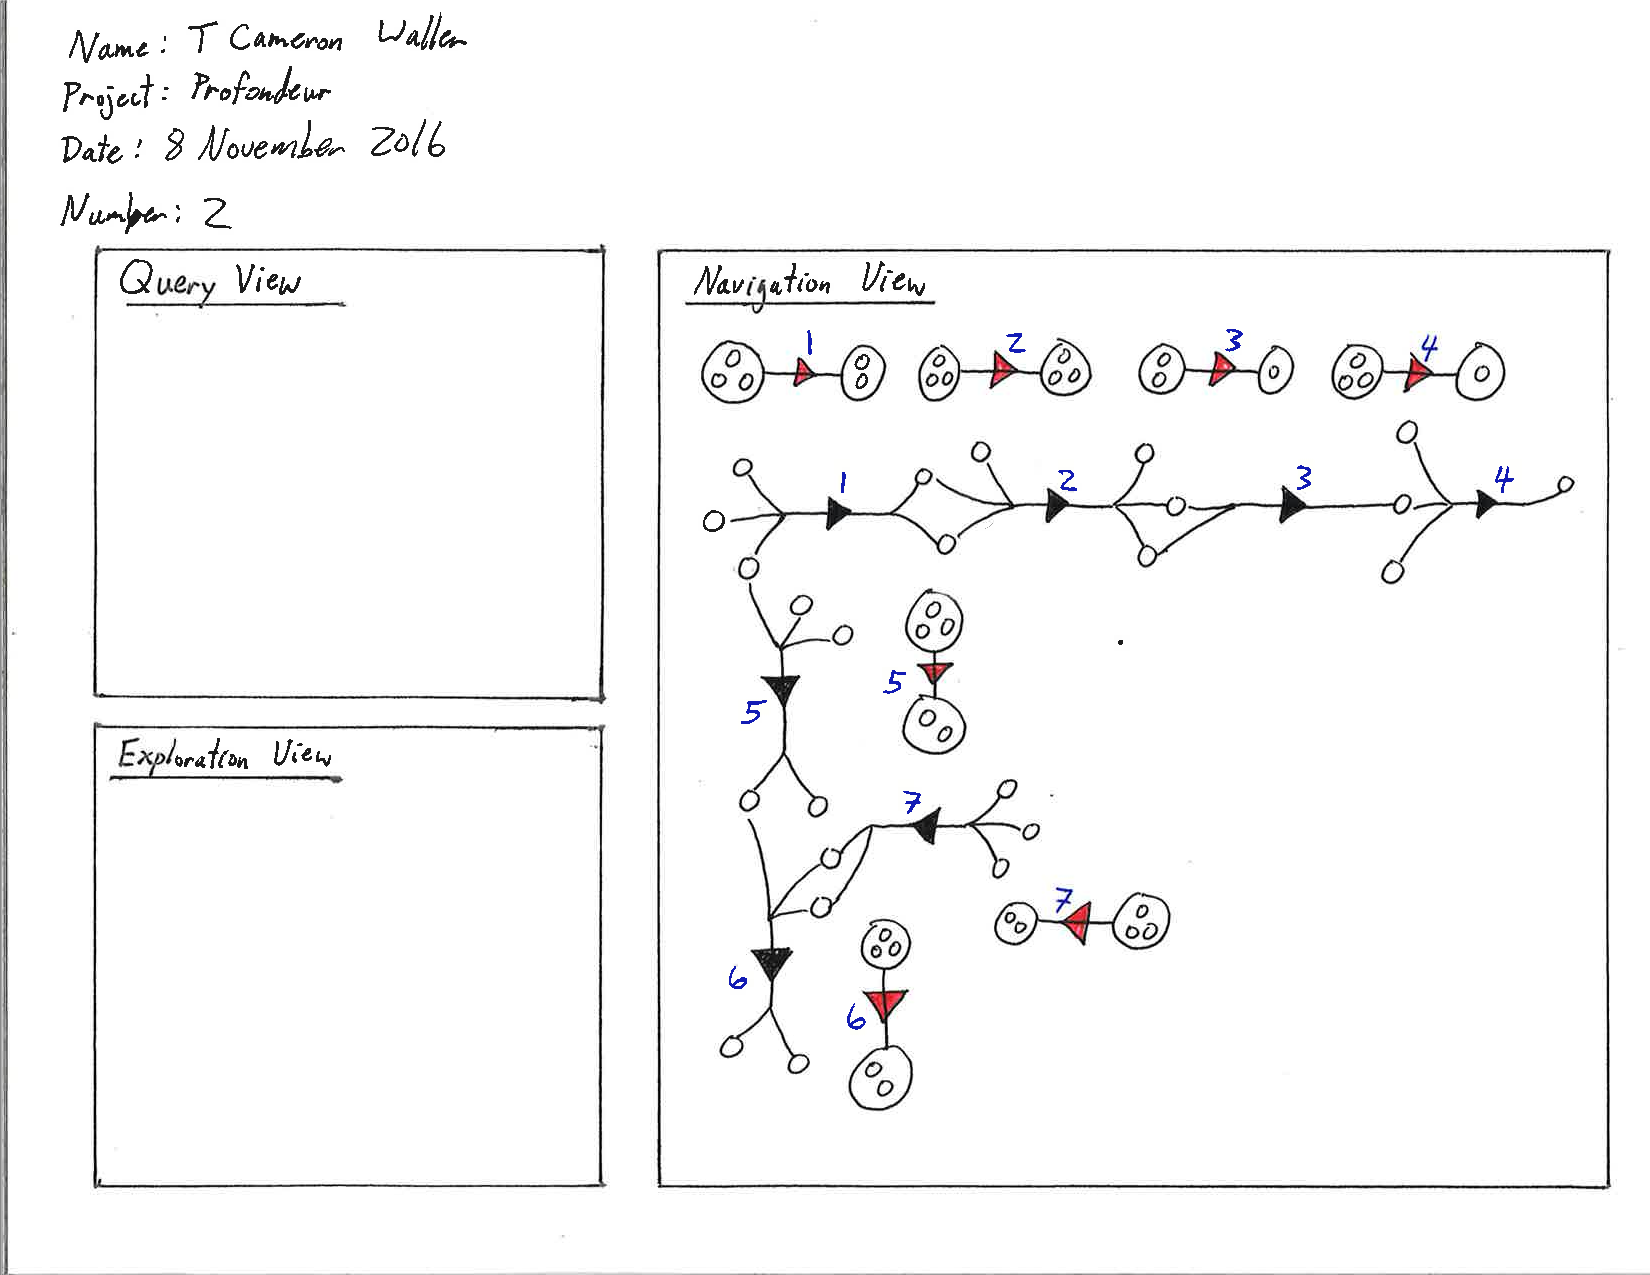
\includegraphics[scale=0.5]{sketch_2016-11-08_2}
\centering
\caption{Problem with super nodes for reactant and product metabolites}
\label{fig:2016-11-08_2}
\end{figure}

\begin{figure}[t]
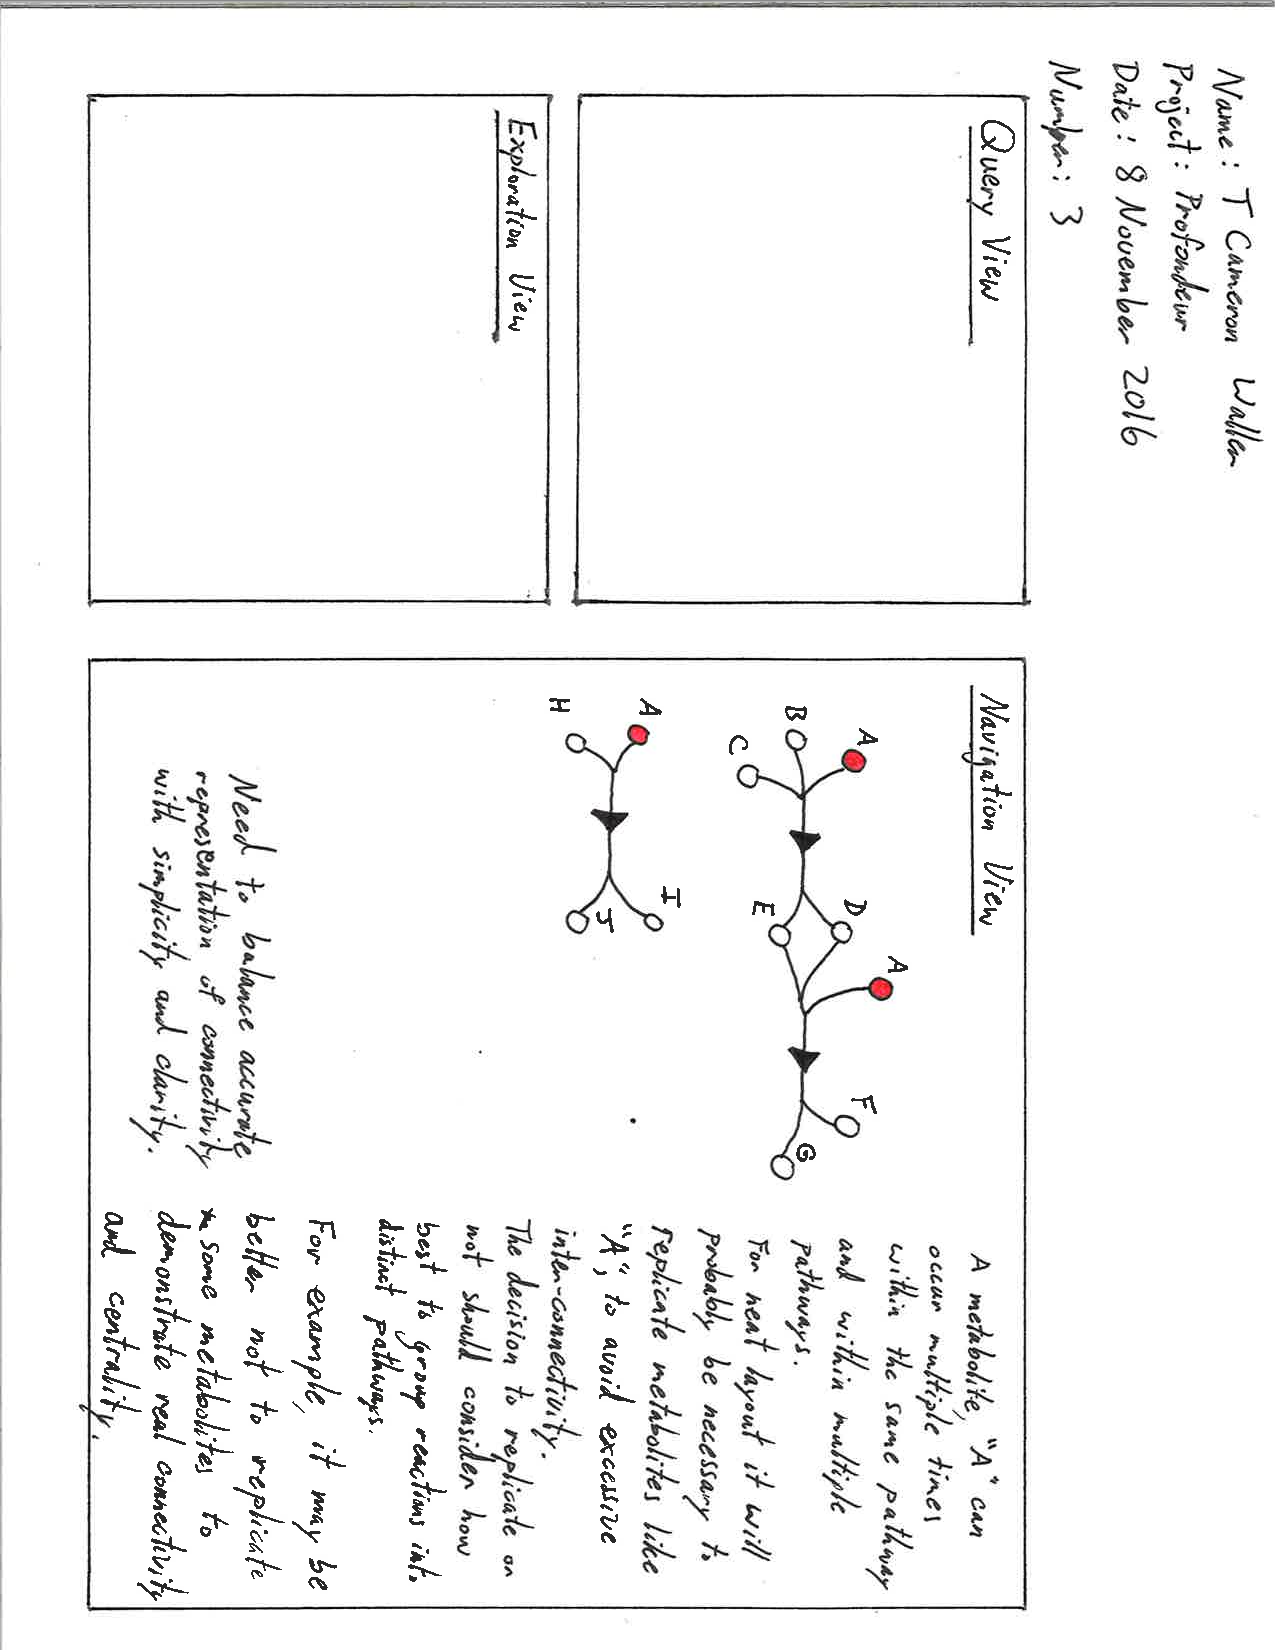
\includegraphics[scale=0.5]{sketch_2016-11-08_3}
\centering
\caption{Replication of high-degree nodes to simplify network}
\label{fig:2016-11-08_3}
\end{figure}

\begin{figure}[t]
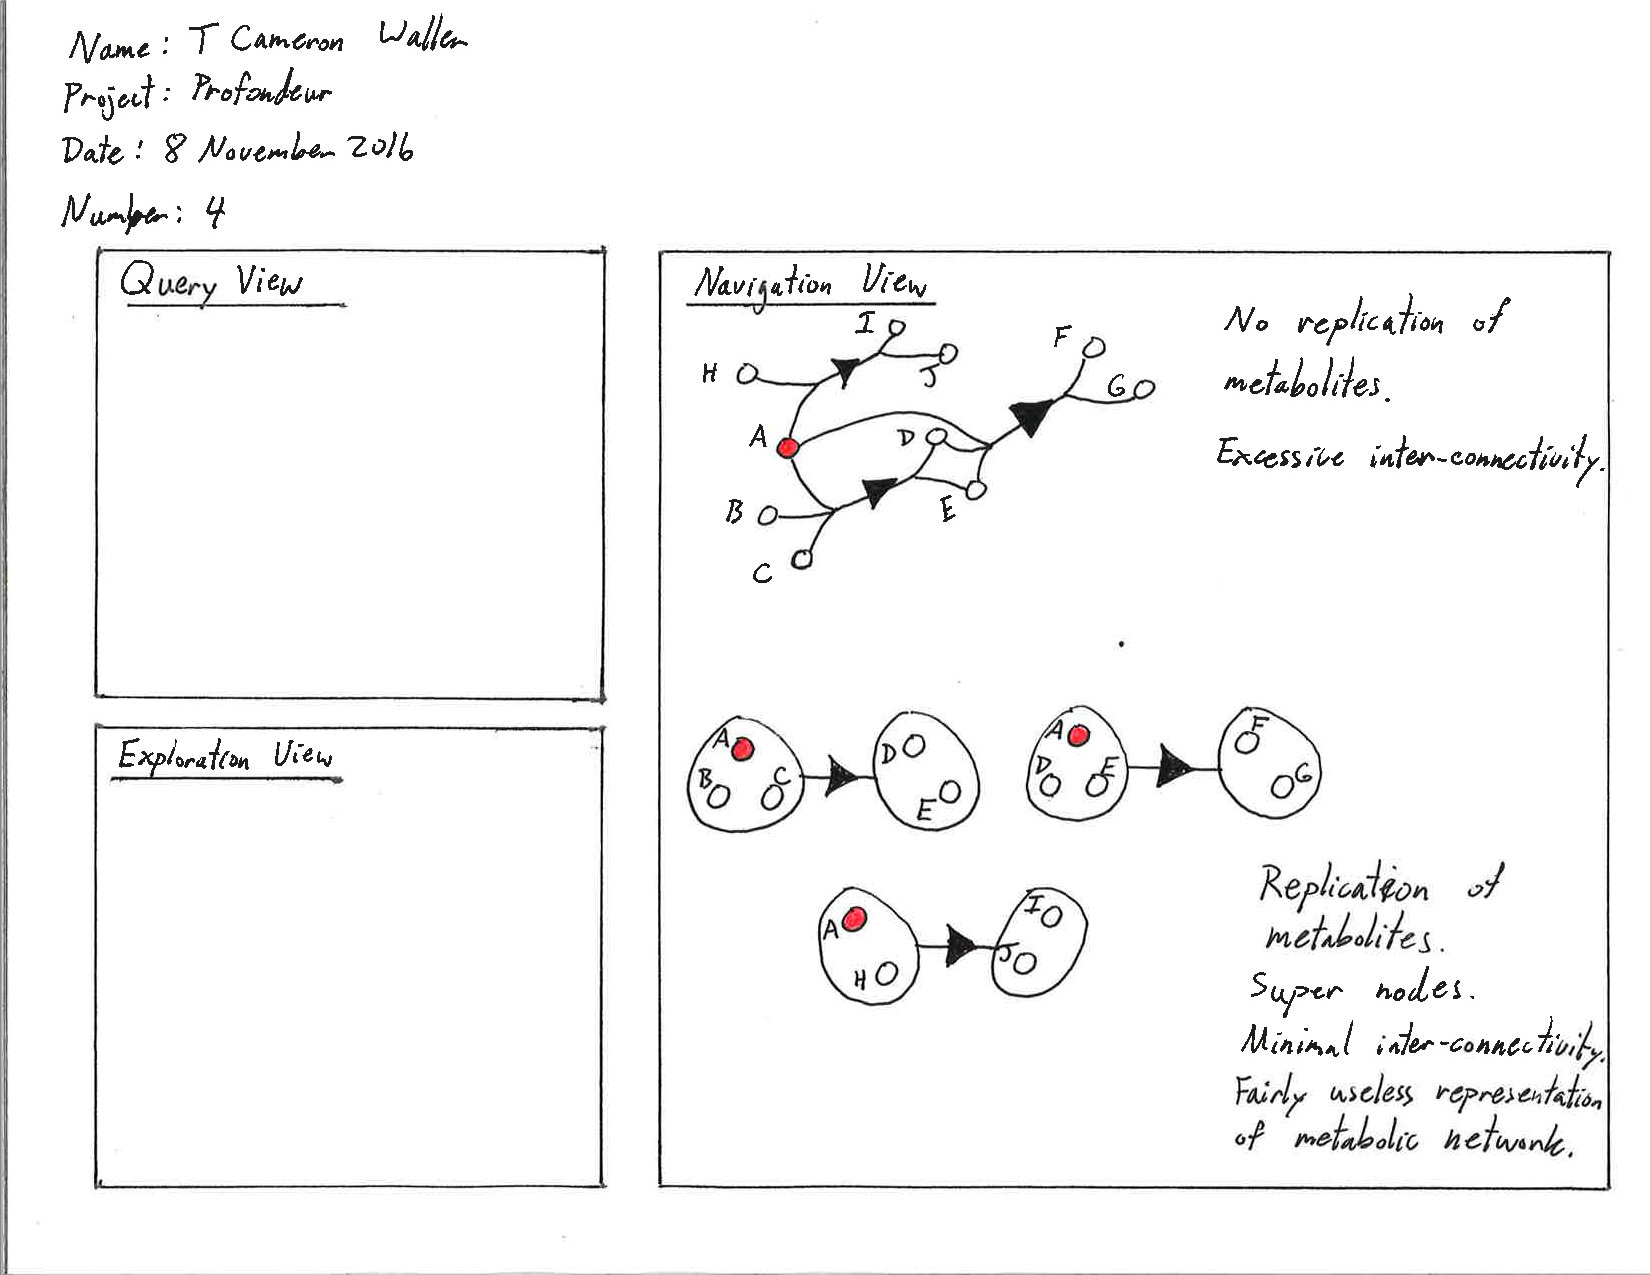
\includegraphics[scale=0.5]{sketch_2016-11-08_4}
\centering
\caption{Preservation of connectivity in the network}
\label{fig:2016-11-08_4}
\end{figure}

\begin{figure}[t]
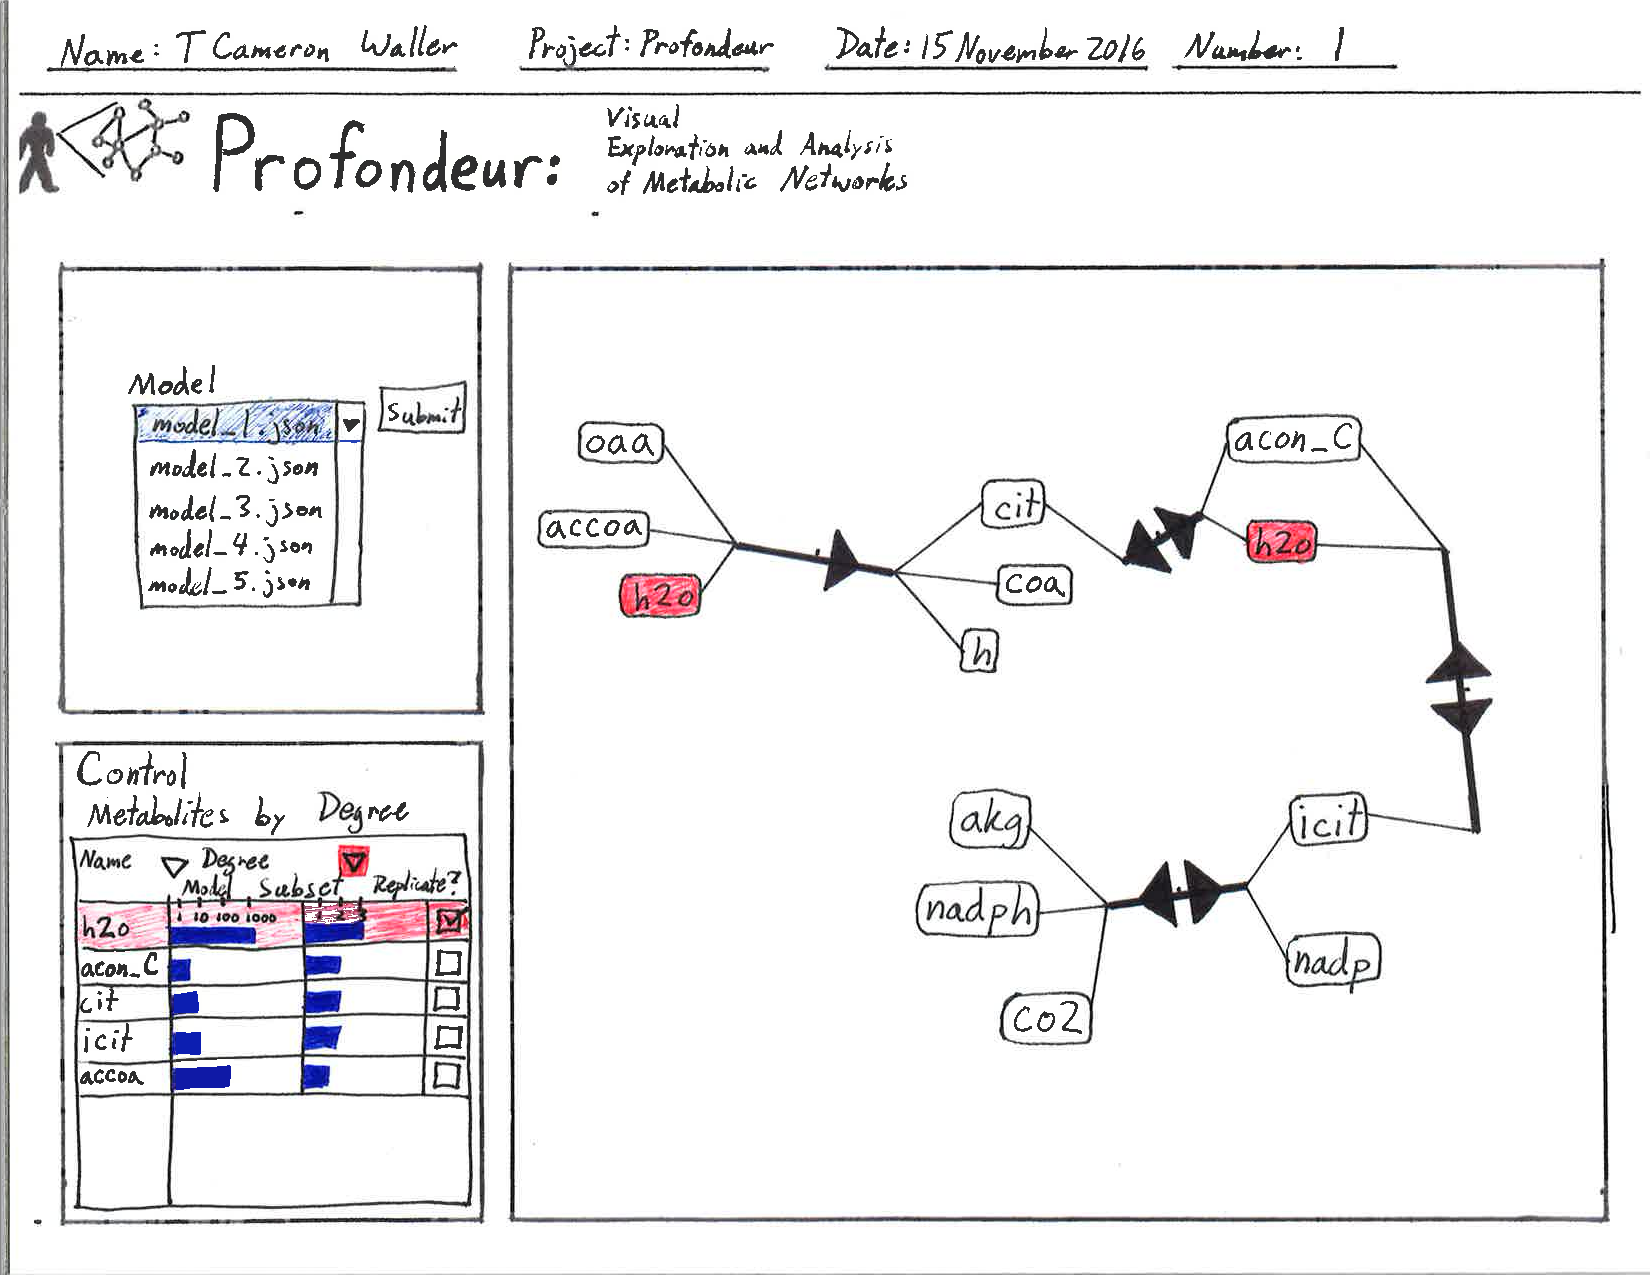
\includegraphics[scale=0.5]{sketch_2016-11-15_1}
\centering
\caption{User selection of high-degree nodes to replicate}
\label{fig:2016-11-15_1}
\end{figure}

\begin{figure}[t]
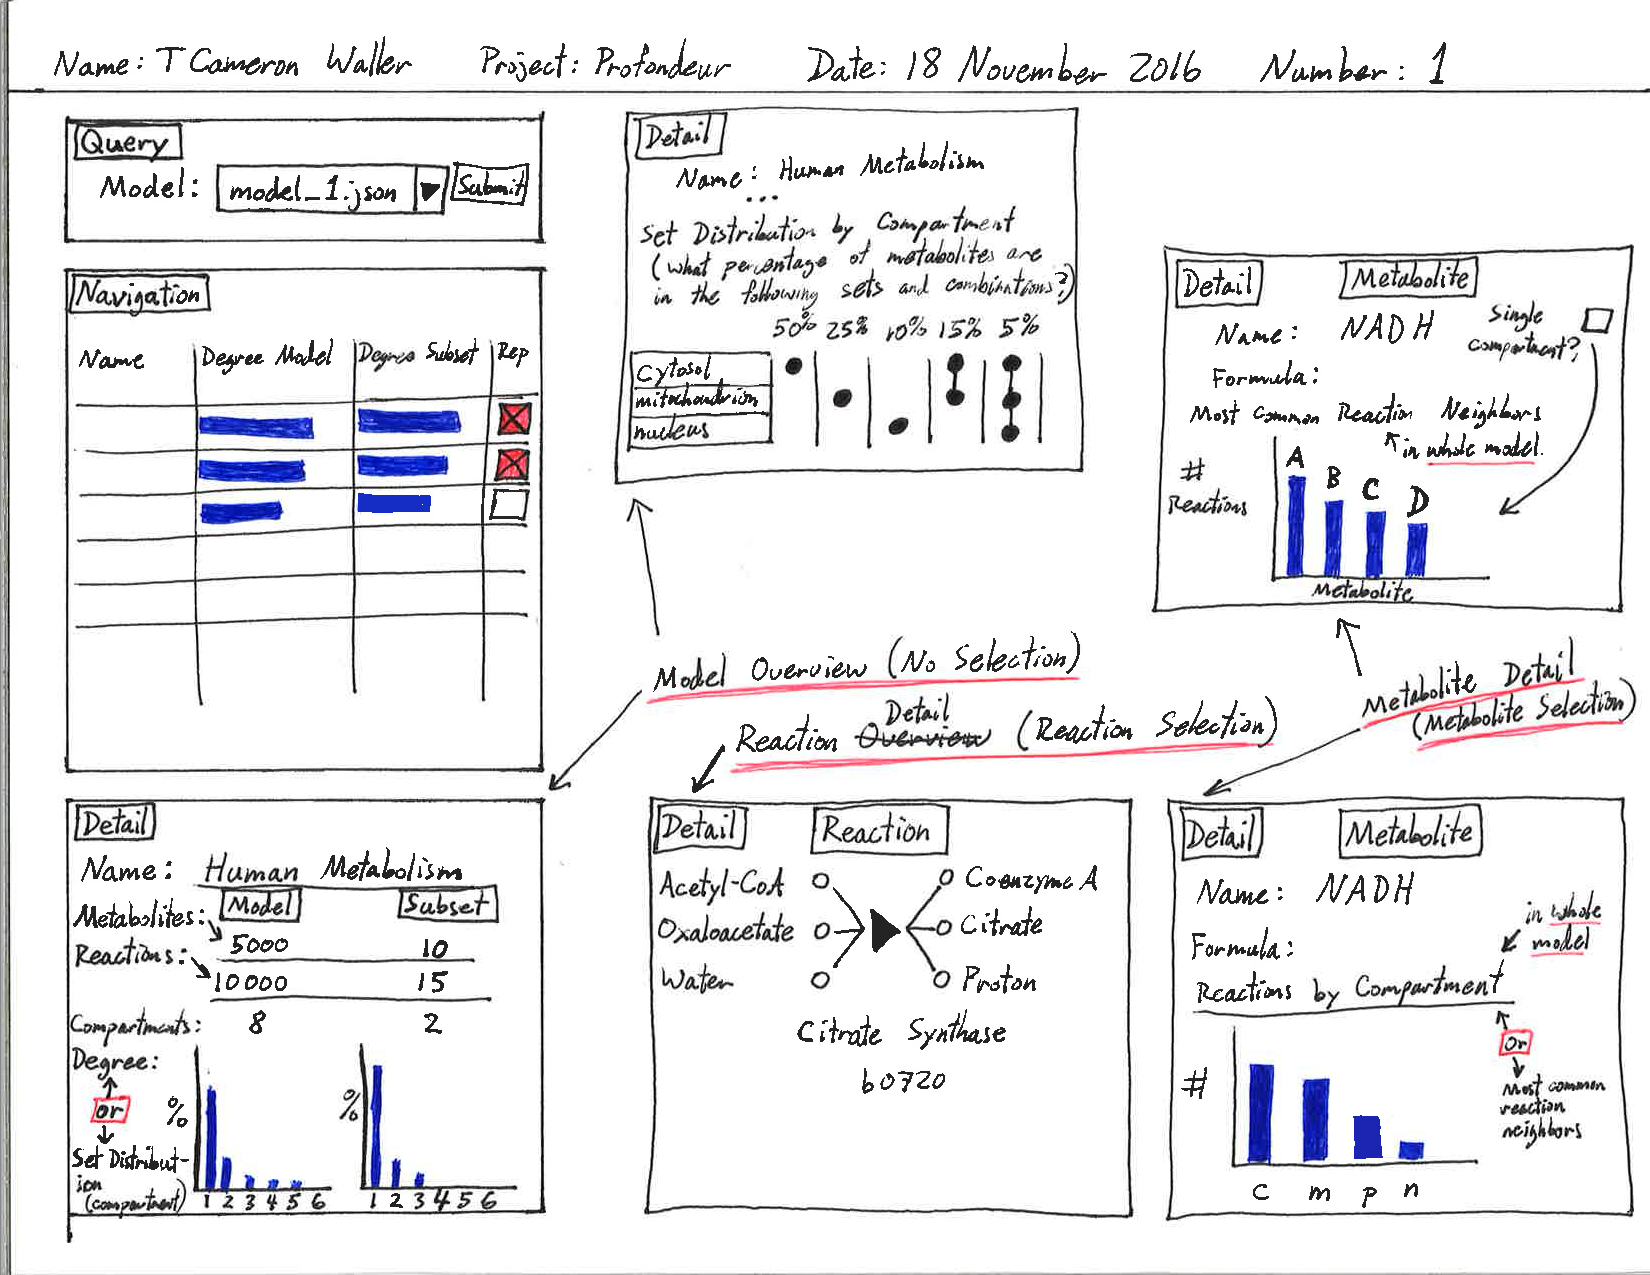
\includegraphics[scale=0.5]{sketch_2016-11-18_1}
\centering
\caption{Detail views with additional information about the network}
\label{fig:2016-11-18_1}
\end{figure}


% Chapter Record

\section{Project Information}
\noindent
\textbf{Project Title:} Profondeur\newline
\textbf{Project Website:} https://tcameronwaller.github.io/profondeur/\newline
\textbf{Project Repository:} https://github.com/tcameronwaller/profondeur\newline
\textbf{Author Name:} Thomas Cameron Waller\newline
\textbf{Author EMail:} cameron.waller@biochem.utah.edu\newline
\textbf{Author Identifier:} 00409400

\section{Introduction}

% Clarify the users, their needs, and their tasks.
% Clarify the scope of this prototype.
% Consider the concept of a Technology Probe (probe the realm of possibility).

The biological study of metabolism has potential to promote the domains of biotechnology, pharmacology, and medicine.
Thereby, this study has potential to benefit human health.
Metabolism is a complex system.
The experimental study of metabolism involves large and complex data sets that are difficult to interpret.
Interpretation requires consideration of the complex metabolic system.
Prospective users are investigators in the domains of biology, biotechnology, pharmacology, and medicine.
These users have very diverse backgrounds and very variable familiarity and expertise in metabolism, and data analysis.

Users need to access information about biological entities and the relations between them.
This information gives relevant context for experimental design and interpretation of experimental results.
This information is especially important for interpretation of large-scale data sets that cover the metabolic system broadly.

\section{Current Technology}

This section includes a concise depiction of the current technology that is relevant to this project with summaries and evaluations of a set of tools.
This set of tools is not comprehensive.

\subsection{Databases}

There are many databases that provide information relevant to the metabolic network.
A few notable examples are the Kyoto Encyclopedia of Genes and Genomes (KEGG, http://www.genome.jp/kegg/) \supercite{kanehisa_kegg_2016}, the MetaCyc Metabolic Pathway Database (http://www.metacyc.org/) \supercite{caspi_metacyc_2016}, and the Universal Protein Resource (UniProt, http://www.uniprot.org/) \supercite{uniprot_consortium_uniprot:_2015}.

\subsection{Metabolic Models}

Systems Biology assembles intricate computational models in order to study cellular functions in a holistic way \supercite{obrien_using_2015, bordbar_constraint-based_2014}.
Communities of scientists thoroughly assemble and maintain computational models that comprise current knowledge of the metabolic systems of multiple species.
A current model of high quality is available for human metabolism \supercite{thiele_community-driven_2013, swainston_recon_2016}.

\subsection{Visualization and Exploratory Analysis}

KEGG Atlas (http://www.kegg.jp/kegg/atlas/) \supercite{kanehisa_kegg_2016} is a web application that enables users to explore metabolic maps from KEGG.
The user can select from a large set of available maps for subsets and pathways in metabolism.
Maps in the atlas use a static, spatial layout that sometimes distorts the relations between metabolites.
Two metabolites may be far apart on the map although they relate by a single reaction.
The atlas also does not allow the user to specify custom subsets of the network.
This design renders KEGG Atlas inappropriate for visualizing subsets of the metabolic network that traverse typical pathways.

Escher (https://escher.github.io/) \supercite{king_escher:_2015} is a web application that enables users to draw metabolic maps and visualize experimental data on these maps.
It imports information from models of metabolism that the systems biology community develops and maintains, thereby favoring accuracy, and allows the user to select portions of these models to include in the maps.
Escher's fundamental design requires the user to select portions of the metabolic model and position these in a static layout.
This design renders Escher inappropriate for a query-based exploration system that would need to represent automatically and dynamically a broad variety of custom subsets of the metabolic network.

\section{Problems/Objectives}

% Give more specifics on the tasks or questions.

\section{Problems}

How is it possible to represent the metabolic network accurately and clearly using custom subsets of the network and automatic layouts of node-link graphs?

Users often have sets of multiple entities (metabolites, proteins, transcripts, genes) of interest, such as those for which they have experimental data, in the metabolic system.
Users need to know how these entities relate to each other.
Many of these relations transcend or traverse typical, common, traditional pathways.
There are many dimensions, levels, or layers of relations in the metabolic system.
At the most basic level, users need to know how multiple metabolites relate to each other through chemical reactions.
These reactions are a single dimension of the metabolic system.
Types of entities other than metabolites also participate in this dimension of the metabolic system.
Users need to know the proteins that either catalyze reactions or transport metabolites between cellular compartments.
Users need to know the transcripts and genes that encode these proteins.

Users also need to know about properties that might be relevant to relations between entities.
Maybe multiple entities share a property.
These properties might inform biological interpretation.

Data about the metabolic system describe properties of and relations between genes, transcripts, proteins, and metabolites.
Experimental data describe modifications to genes, transcripts or proteins.
Experimental data also describe the abundances of transcripts, proteins, or metabolites.

In the most common use scenario, the user needs to interpret data for a single type of entities, such as metabolites.
In a higher-level use scenario, the user needs to interpret data for two types of entities simultaneously, such as metabolites and transcripts.

The metabolic system is large and complex.
It is impractical, unreasonable, and useless for a human user to attempt to conceptualize the entire system simultaneously.
The user needs methods to select subsets of the metabolic system that are relevant to the user's interest (such as an experiment).
This selection process itself might involve many criteria and be complex.
Methods for this selection are excellent design opportunities.
Many possible factors could influence their effectiveness.

Even subsets of the metabolic system might be excessively complex.
The user needs methods to explore these subsets.
The user needs to recognize important information from the metabolic system easily.
The user needs a summary or overview to give context.
The user needs details on demand or details according to interest.
Methods for this exploration are excellent design opportunities.

Experimental data convey information about entities in the metabolic system.
Users need methods to recognize trends in these data that are dependent on aspects of the metabolic system.
Methods for this data communication are excellent design opportunities.

\section{Data}

Systems biology is a mature sub-domain of biology that considers and studies biological systems from an holistic perspective.
This sub-domain commonly develops intricate mathematical models and uses these in computational simulations.
These models include information about metabolites (the small molecules of metabolism), chemical reactions between them, the rates and directionality of these reactions, the cellular compartments where these reactions happen, the protein enzymes that catalyze these reactions, and the transcripts and genes that encode these proteins.
The ultimate goal is for these models to represent the entirety of the biological system, and many models are comprehensive collections of current biological knowledge.

An active community in systems biology develops and curates these metabolic models as well as develops and maintains extensive resources for using them.
The Systems-Biology-Markup-Language (SBML) (http://sbml.org) relates to the Extensible-Markup-Language (XML) and is an open standard and format for the representation of computational models for biological systems.
Robust models in SBML are available for the metabolic systems of many organisms, including \textit{Mus musculus} (mouse) and \textit{Homo sapiens} (human).
For this project, I chose to derive data from these metabolic models because they represent the most comprehensive and orderly (mass and charge-balanced reactions, compartments) collections of current biological knowledge on the metabolic system.

COBRApy (https://opencobra.github.io/cobrapy/) \supercite{ebrahim_cobrapy:_2013} is an open-source tool from the community for using metabolic models in Python.
I will use COBRApy along with libSBML (http://sbml.org/Software/libSBML) \supercite{bornstein_libsbml:_2008} to convert data for metabolic models from SBML format to JavaScript Object Notation (JSON) format.
I will use these data in JSON format in the web application, ultimately restructuring it for graph queries and representation in node-link graphs.
To pilot the prototype of this web application, I used a small model of central metabolism in \textit{Escherichia coli} (Gram-negative bacterium) that came as a model for demonstration in COBRApy.
I modified this model to simplify it and derived the appropriate structure of nodes and links manually.

\section{Exploratory Data Analysis}

% Describe the process of coming to understand the data, such as what information the data includes, the characteristics.
% Explain the selection of subsets of the data for illustrative purposes.
% Explain how I interacted with the data in its original/early form.


I am familiar with the metabolic network and visual representations of it from various sources.
These include databases and charts that I mentioned in Section "Related Work".
I have also drawn many of my own visual representations of the metabolic network using InkScape.
I gathered information for these representations from databases such as KEGG, MetaCyc, and UniProt.

For this project, I specifically use data from metabolic models.
The structure of these data was less familiar to me.
I explored metabolic models to learn about the information that they include and how to interpret this information correctly.
I used COBRApy (ref) for this exploration of the raw data from the metabolic model.
I also used a visual editor (http://www.jsoneditoronline.org/) to examine the metabolic model in JSON format.

\section{Design}

% Only mention the high-level ideas.
% Maybe include an appendix to document all of the sketches and the complete evolution of design in the project.

This project's repository (https://github.com/tcameronwaller/profondeur) has a directory with title "design".
Within this directory are scans of sketches that I drew or recorded during the design process.
Also in this directory is a text file with title "note sketch".
This file contains notes on several important or influential sketches and the relevant design concepts.

\subsection{Network of Multiple Dimensions}

I began the design process with a grand idea of the complexity of the biological system and the metabolic network within this system.
In reality, the metabolic network involves multiple types of entities (genes, transcripts, proteins, metabolites) and multiple types of relations between them (encoding, expression, regulation, transport, catalysis, reaction).
All of these entities and relations have their own properties that may be interesting in a biological context.

I had a multidimensional or multilayer network, and I needed to figure out how to visualize it.
I sketched several ideas for how to represent this multidimensional network, as Figures \ref{fig:2016-10-11_2}, \ref{fig:2016-10-11_3}, \ref{fig:2016-10-31_1}, illustrate.
I even considered alternative types of charts in order to accommodate the complexity as Figures \ref{fig:2016-10-11_4} and \ref{fig:2016-10-31_3} illustrate.
I imaged that an interface might look something like Figure \ref{fig:2016-10-20_1} illustrates.

\subsection{Network of Reactions between Metabolites}

Eventually, on 1 November 2016, I consulted with a domain expert in the biological study of metabolism, Jared P Rutter.
Jared encouraged me to begin with a network of reactions between metabolites in order to simplify the problem.
I considered designs to illustrate reactions between metabolites.

I decided to represent metabolites as nodes and reactions as links between those nodes.
Around that time, as I interacted more with an actual metabolic model, I realized that multiple metabolites can participate as reactants or products of the same reaction.
From my background in biology, I already knew that, of course, but I suppose I had not really considered how to accommodate that complexity in the network representation.
To simplify, I considered using either link bundles or super links as Figure \ref{fig:2016-11-07_1} illustrates.
I also considered the idea of using super nodes for reactant and product metabolites as Figure \ref{fig:2016-11-08_1} illustrates, but I realized that super nodes would abolish much of the connectivity of the network as Figure \ref{fig:2016-11-08_2} illustrates.

\subsection{Node Replication for Prolific Metabolites}

As I worked with the data for the metabolic model more, I realized that the metabolic network can be very complex because some metabolites are very prolific.
A single metabolite can participate as a reactant or product in multiple reactions.
It can simplify the representation of the network to replicate the nodes for these prolific metabolites, as Figure \ref{fig:2016-11-08_3} illustrates.
In contrast, it is a more accurate representation of the connectivity of the network to preserve the centrality of these metabolites, as Figure \ref{fig:2016-11-08_4} illustrates.
The connectivity of some prolific metabolites (pyruvate) might be more interesting than that of some other metabolites (such as water, proton, carbon dioxide, ADP, ATP, NAD, NADH, NADP, NADPH).
I decided that it would be beneficial to allow the user to decide whether or not to replicate nodes for metabolites.
My final design sketch, Figure \ref{fig:2016-11-15_1} illustrates a table interface to allow the user to select metabolites with high-degrees to replicate.

\subsection{Future Goals}

Figure \ref{fig:2016-11-18_1} illustrates some of my ideas for future goals.
The idea is to provide the user with more information about the network according to the user's interest and selections.

\section{Implementation}

I implemented the design that Figure \ref{fig:2016-11-18_1} illustrates (with the exception of showing degrees for metabolites in the entire metabolic model since that is beyond scope).
I implemented this interface as a web application using Hyper Text Markup Language (HTML), Cascading Style Sheets (CSS), and JavaScript.
The code is available in the project repository (https://github.com/tcameronwaller/profondeur), and a demonstration of the interface is available as a website (https://tcameronwaller.github.io/profondeur/).

\section{Evaluation}

The prototype demonstrates the feasibility of using an automatic and dynamic layout algorithm to represent node-link diagrams of subsets of the metabolic network.
Such layout algorithms are necessary to allow users to visualize custom subsets that they define through queries.
The prototype also demonstrates the utility in enabling the user to select which (if any) nodes to replicate in the network.
The decision to replicate nodes balances accurate representation of the network against simplification of this representation.
The decision really depends on the interest of the user, and I think it is best to leave it to the user.

Within the scope of the project, I consider the prototype to solve some important problems, and to consider some of the most critical requirements of this project.
In order to progress further, it was very important to evaluate the feasibility of automatic, dynamic layouts of subsets of the metabolic network from custom queries.
Now that this layout is a possibility, the project can progress in the future.